\section{Results}
\label{sec:results}

\subsection{Criticalities}

The main goal of GOFR was to test the feasibility of a geometric approach to research reactors and to fit the resultant reactor into the size of a room. This dimensional criteria was where calculations started. Various sizes of cubes, for ease of visualization, were tested, to get a sense of how criticality scaled with size and how large the final core would be. From the below table, it is seen that criticality rises linearly with volume. Since a self sustaining reaction requires a k-coefficient of $k=1$ that is what was tested for. It also shows the maximum moderated potential of each core because the many meters of water completely stopped all neutron activity outside its bounds.

\begin{table}[!htbp]
\centering
\caption{U-235 core trials}
\label{tab:pureU}
\begin{tabular}{|c|c|c|c|}
\hline
Composition & cc of U-235 		& Moderator	& k-coefficient  \\
\hline
U-235  		&  1000             & Vacuum	& 0.74311     \\
\hline
U-235  		&  1000             & Water     & 1.26001     \\
\hline
U-235  		&  8000             & Vacuum    & 1.30614     \\
\hline
U-235  		&  8000             & Water     & 1.49408     \\
\hline
U-235  		& 27000             & Vacuum    & 1.64085     \\
\hline
U-235  		& 27000             & Water     & 1.76348     \\
\hline
\end{tabular}
\end{table}

Table \ref{tab:pureU} suggests that a volume greater than a thousand cube centimeters of U-235 is needed for sustained fission, unless heavily moderated, but eight thousand is excessive. These initial results provide a good place to start experimenting with lower enrichments and different alloys. First, a conventionally designed reactor was designed, to provide an initial criticality and flux value. Different core sizes and enrichments were tried, submerged in water, in a graphite flask. A 15\% enriched uranium core of 30 square centimeters was decided upon.

\begin{table}[!htbp]
\centering
\caption{Conventional Reactor variations}
\label{tab:variations}
\begin{tabular}{|c|c|c|c|}
\hline
Composition            & Side length (cm)	& cc of U-235	& k-coefficient \\
\hline
20\% enriched Uranium  & 10               	&   200			& 0.85447       \\
\hline
20\% enriched Uranium  & 20               	&  1600			& 1.02792       \\
\hline
20\% enriched Uranium  & 30               	&  5400			& 1.15384       \\
\hline
20\% enriched Uranium  & 60               	& 43200			& 1.40225       \\
\hline
15\% enriched Uranium  & 60               	& 32400			& 1.27469       \\
\hline
15\% enriched Uranium  & 40               	&  9600			& 1.15583       \\
\hline
15\% enriched Uranium  & 30               	&  4050			& 1.06625       \\
\hline
\end{tabular}
\end{table}

Four cores were devised to test things further. The first two were differently enriched uranium cores, 80\% and 20\%, designated HEU and LEU, respectively. The last two are alloys of half LEU and a metal, zirconium hydride and aluminum. These are designated as $UZrH_4$ and UAl, respectively. A sphere of $r=10cm$ was assumed, as spheres should better utilize generated neutrons and the volume of a sphere increases rapidly with radius. The intention was to make the core go critical with the optimized shell and the core alloys.


\begin{table}[!htbp]
\centering
\caption{Core criticality testing, $r=10cm$}
\label{tab:kcore}
\begin{tabular}{|c|c|c|}
\hline
Composition		& cc of U-235		& k-coefficient \\
\hline
HEU	  	        & 3351.03           & 1.04706       \\
\hline
LEU				&  837.76           & 0.51117       \\
\hline
$UZrH_4$ 		&  418.87           & 0.28084       \\
\hline
UAl 			&  418.87           & 0.27939       \\
\hline
\end{tabular}
\end{table}

Table \ref{tab:kcore} shows that with half the uranium, UAl at 54.66\% of the criticality of the LEU core. $UZrH_4$ performs at 54.94\%. Both clearly do something but $UZrH_4$ does more of it. The underlying theory is that the hydrogen in the $UZrH_4$ moderates the energy of the neutrons so that they cause more fissions. This capture is delicate and a rise in temperature that is too high will let neutrons escape the core and force a lower power level. This is the intended function, which is why $UZrH_4$ is included, despite only a slight improvement.

\begin{table}[!htbp]
\centering
\caption{Core+Moderator criticality testing, $r=10cm$}
\label{tab:kmod}
\begin{tabular}{|c|c|c|}
\hline
Composition		& cc of U-238		& k-coefficient \\
\hline
HEU	  	        & 3351.03           & 1.19440       \\
\hline
LEU				&  837.76           & 0.59913       \\
\hline
$UZrH_4$ 		&  418.87           & 0.34255       \\
\hline
UAl 			&  418.87           & 0.34051       \\
\hline
\end{tabular}
\end{table}

The scattering lengths of various moderator materials was studied and it was determined that aluminum would have the smallest interaction with the neutrons while if scatter occurred, it would be elastic. Criticality rose more than expected with the addition of the aluminum moderator in Table \ref{tab:kmod}. There also seems to be a growing disparity between UAl and $UZrH_4$, which is a positive indication of the passive safety features from using $UZrH_4$.

\begin{table}[!htbp]
\centering
\caption{Final criticality testing}
\label{tab:kmod}
\begin{tabular}{|c|c|c|}
\hline
Composition			& cc of U-238		& k-coefficient \\
\hline
HEU	  	        	& 3351.03           & 1.28998       \\
\hline
LEU					&  837.76           & 0.67885       \\
\hline
$UZrH_4$ 			&  418.87           & 0.44506       \\
\hline
UAl 				&  418.87           & 0.44983       \\
\hline
$UZrH_4$ @ 25cm 	& 6544.98           & 1.00546       \\
\hline
\end{tabular}
\end{table}

It was at this point the GOFR shell design was completed confirmed to be, at least geometrically, optimally configured to send as many neutrons as possible through the beam port. The geometry was coded into MCNP, and the aforementioned cores were put into it and then tested for criticality. Since only the HEU was critical, and it seemed that all cores had reached a plateau in criticality, the $UZrH_4$ was run at $r=25$ to get it to the point where it could sustain itself. Since criticality had been achieved, it was time for the FMESH tally. A grid of tallies throughout the beam port recorded the number of neutrons passing through. 

\begin{table}[!htbp]
\centering
\caption{Flux comparison}
\label{tab:flux}
\begin{tabular}{|c|c|c|c|}
\hline
Reactor			& Average Flux ($n/cm^2$)		& Maximum Flux ($n/cm^2$) & Beam Area ($cm^2$) \\
\hline
UMass Lowell FNI  	        & $1.390*10^11$           & $9.200*10^12$   &  900		\\
\hline
Graphite Flask				& $8.877*10^12$           & $1.692*10^13$   &  900		\\
\hline
GOFR Design 				& $1.963*10^13$           & $5.048*10^13$   & 1963		\\
\hline
\end{tabular}
\end{table}

The two reactors had higher flux than the Lowell Research Reactor, as seen in Table \ref{tab:flux}. These values were calculated for a reactor operating at a power level of 1 MW. Each fission of U-235 releases 202.5 MeV of energy, so by dividing a megawatt by that value, it returns the fissions per second. Each fission results in 2.4 neutrons released on average so multiplying the number of fissions by the average number of generated neutrons per fission returns the total neutrons generated each second in the reactor core. After summing the neutrons that passed through the beam port and dividing by the total neutrons generated in that simulation, a ratio is obtained that indicated the number of neutrons that enter the beam port for every generated neutron. Applying that to the number of neutrons generated each second in the core returns an absolute number of neutrons that will pass through the beam port every second. Dividing that by the cross sectional area of the beam port results in the flux of the reactor. Thus, the flux was obtained and listed in Table \ref{tab:flux}.\\

\begin{figure}[!htbp]
\centering
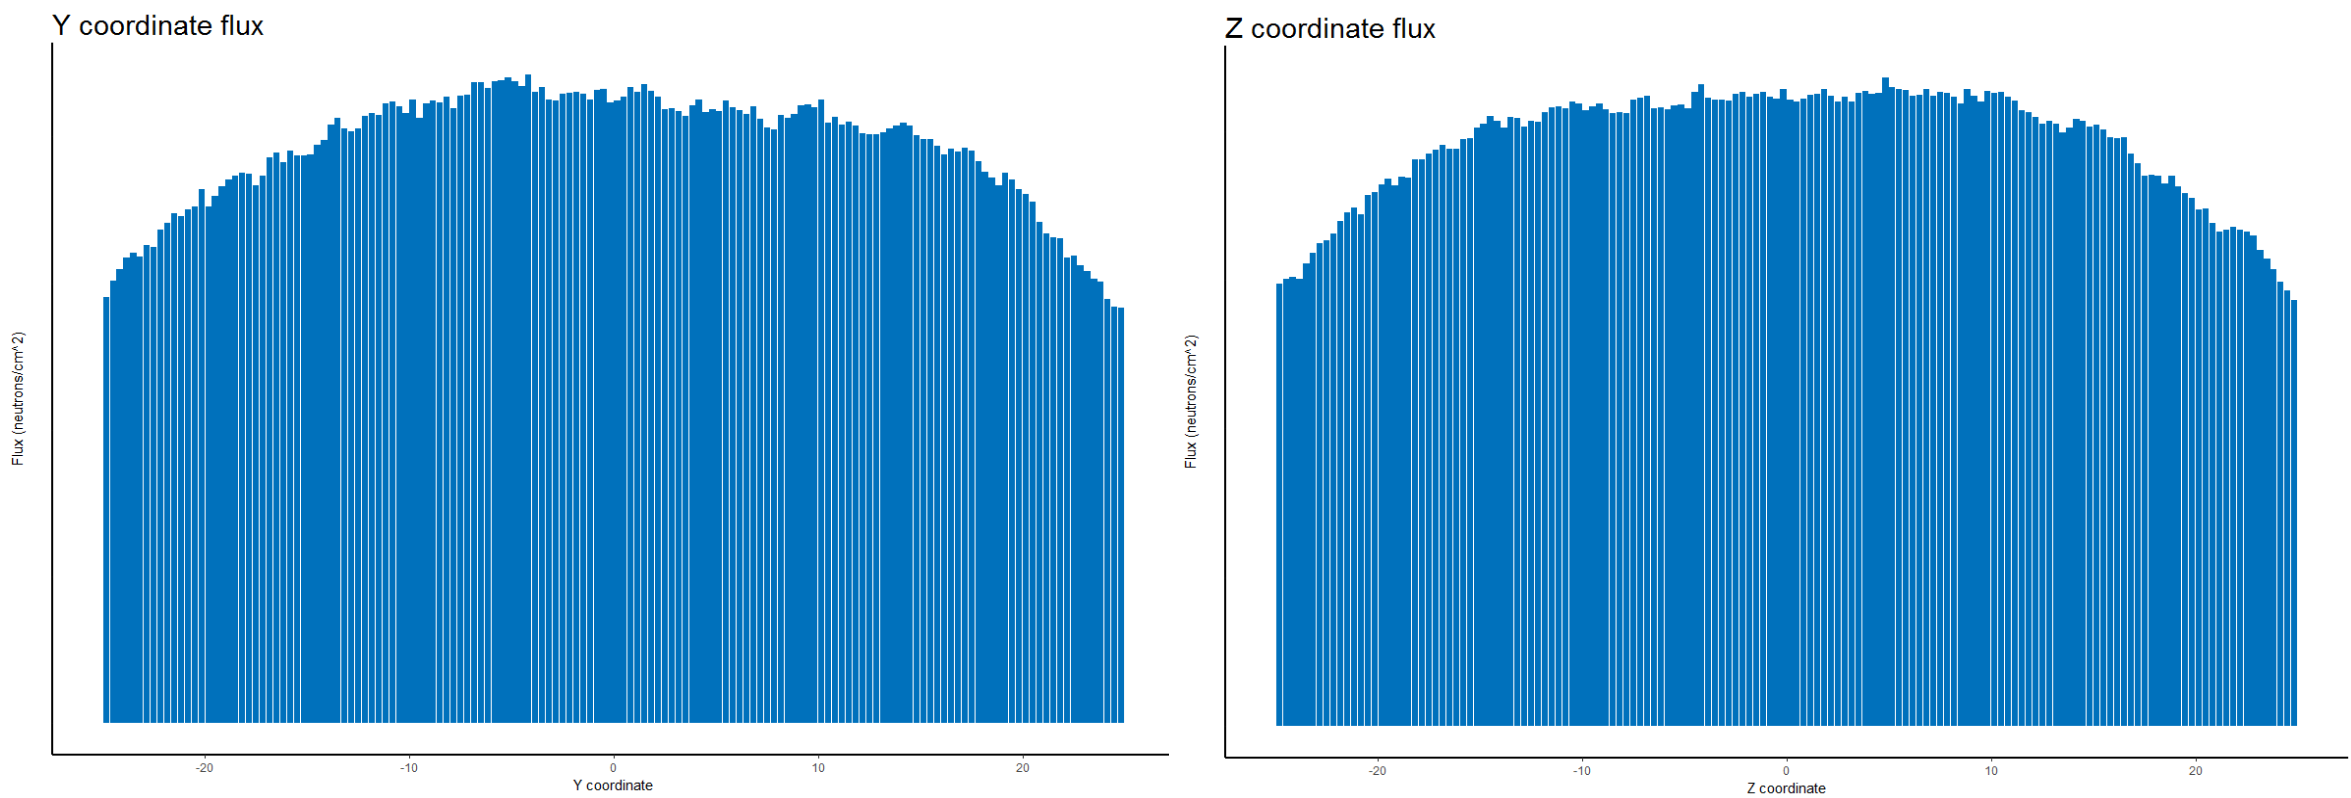
\includegraphics[width=\textwidth]{GOFR_spectrum.png}
\caption{GOFR neutron flux distribution}
\label{fig:GOFR-spec}
\end{figure}

\begin{figure}[!htbp]
\centering
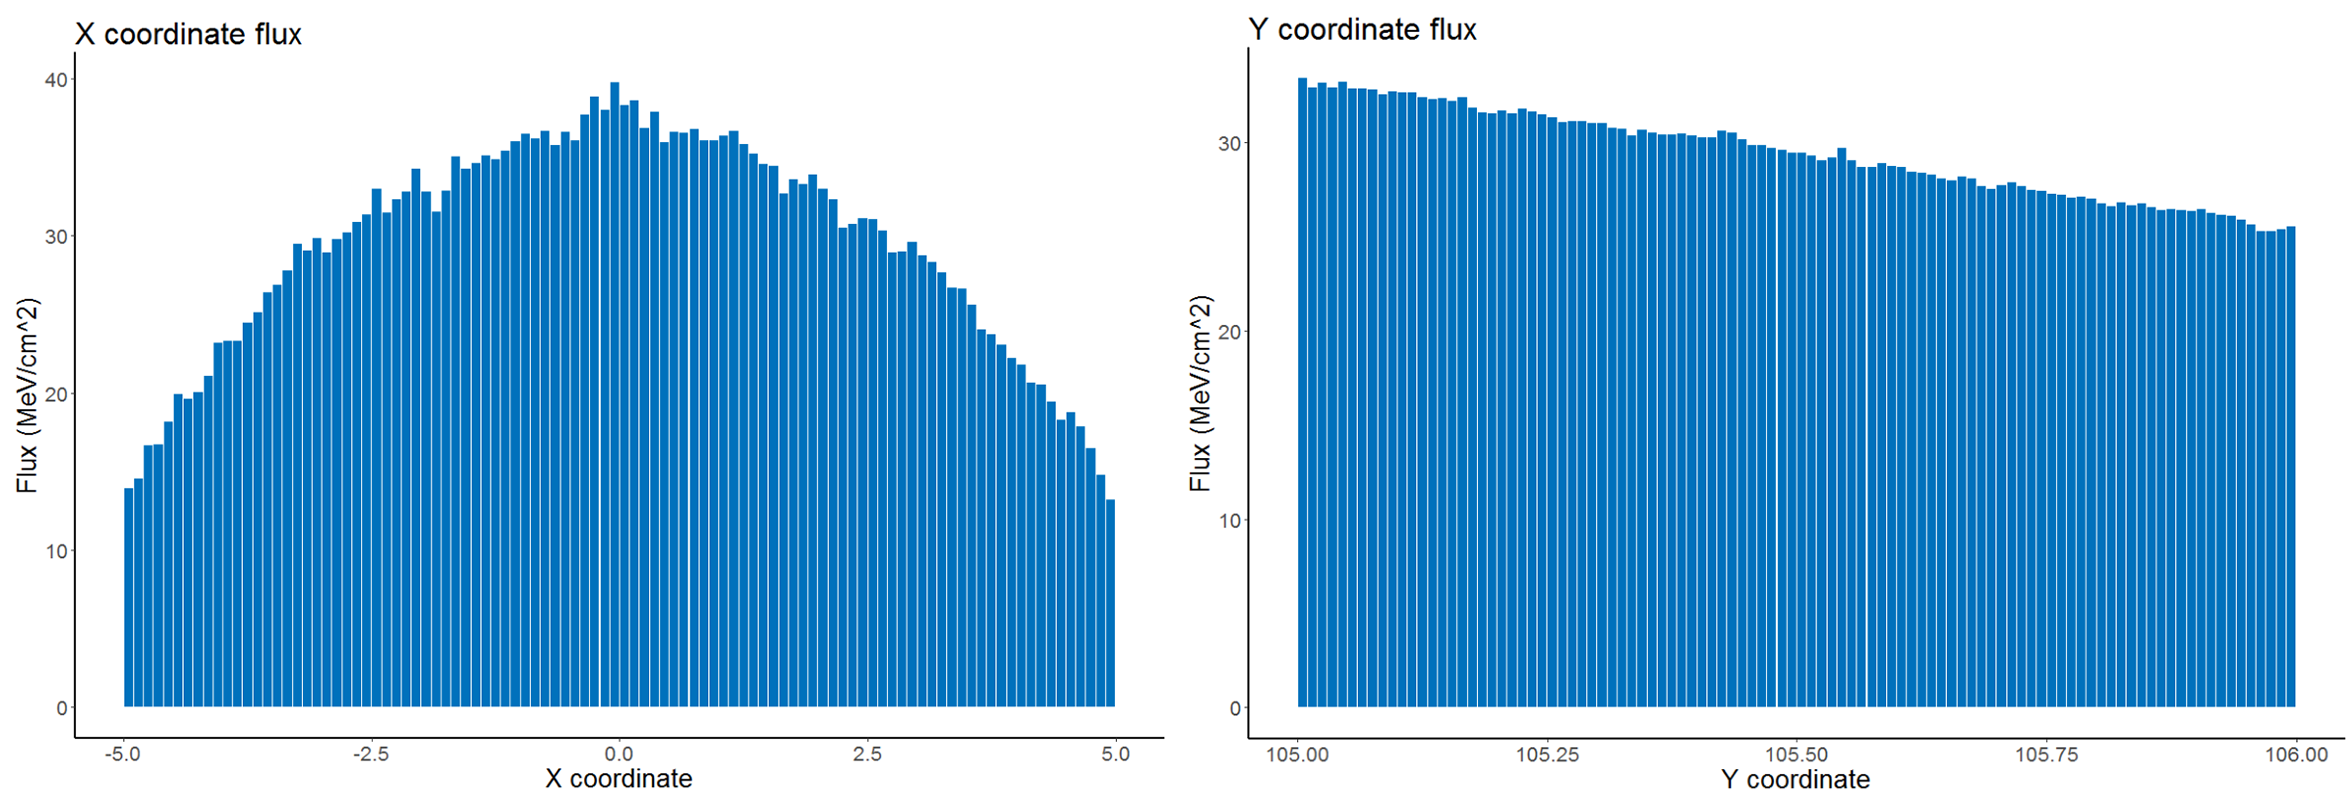
\includegraphics[width=\textwidth]{water_spectrum.png}
\caption{Conventional reactor neutron flux distribution}
\label{fig:water-spec}
\end{figure}

The beam intensity is characterized and shown visually in Figure \ref{fig:GOFR-spec} and Figure \ref{fig:water-spec}, of GOFR and the conventional reactor. This shows that, in addition to having a higher flux, GOFR also has a more uniformly distributed neutron flux, and bigger beam, when compared to the conventional reactor.

\subsection{Reactor designs}
The conventional reactor, the graphite flask of water, design is shown below in Figure \ref{fig:design1}. GOFR, the novel reactor design that was geometrically optimized for high neutron flux is seen below that, in Figure \ref{fig:design2}.

\begin{figure}[!htbp]
\centering
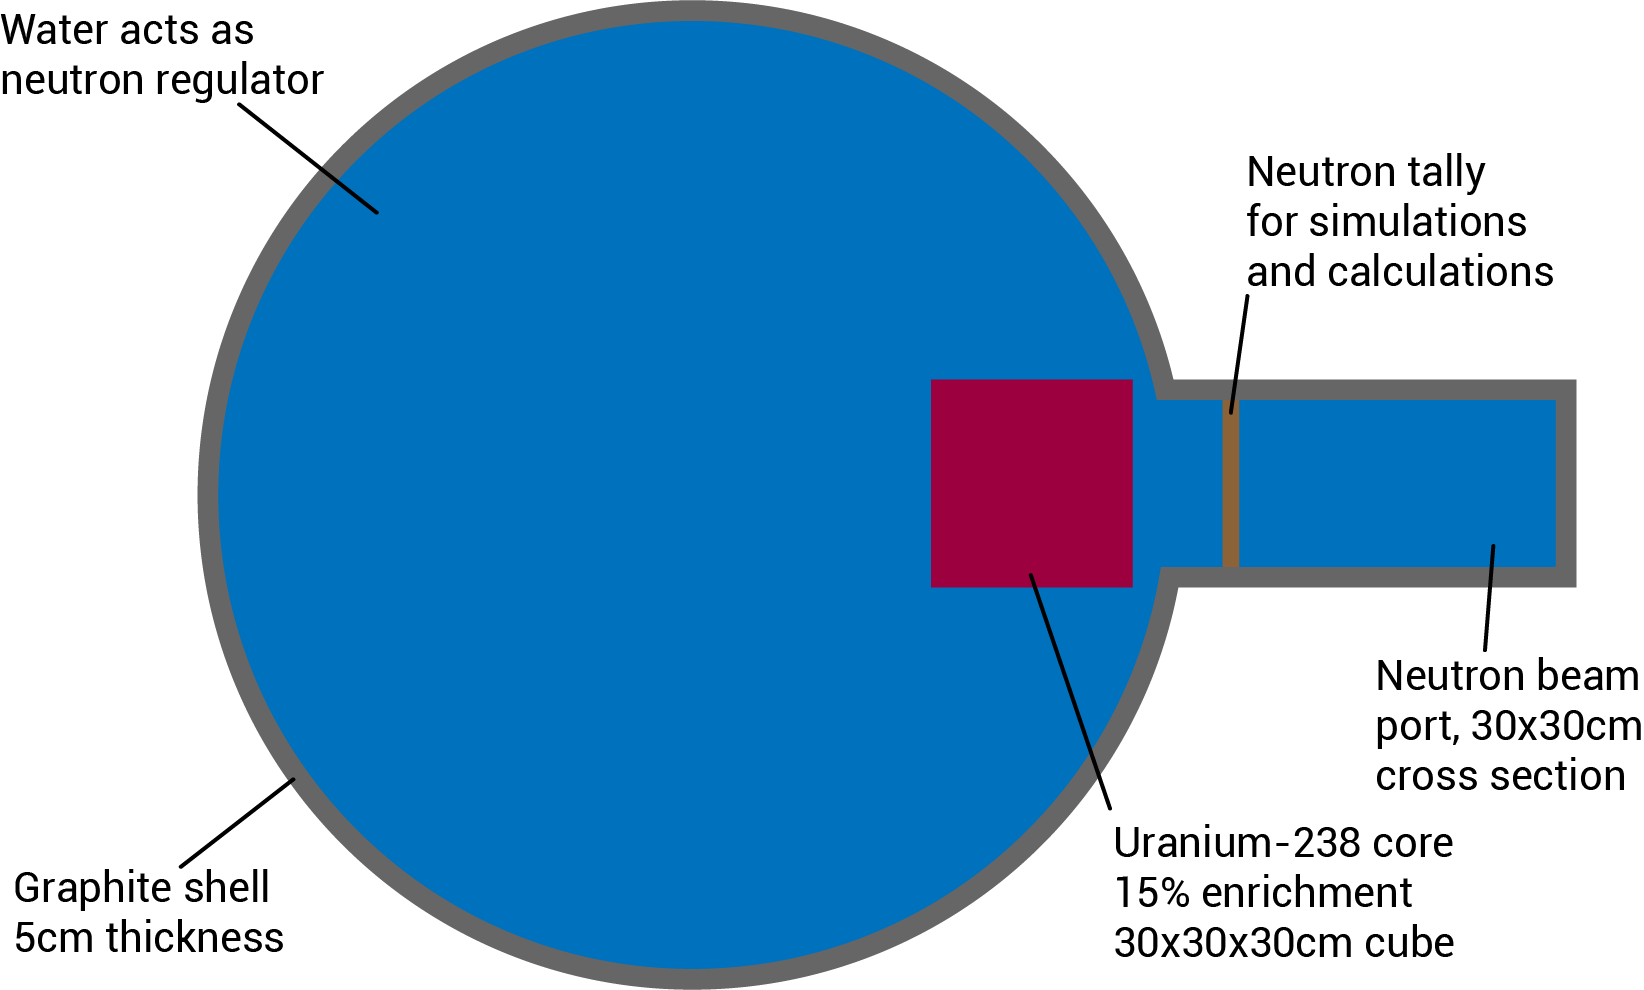
\includegraphics[width=0.75\textwidth]{design.png}
\caption{Conventional graphite flask design}
\label{fig:design1}
\end{figure}

\begin{figure}[!htbp]
\centering
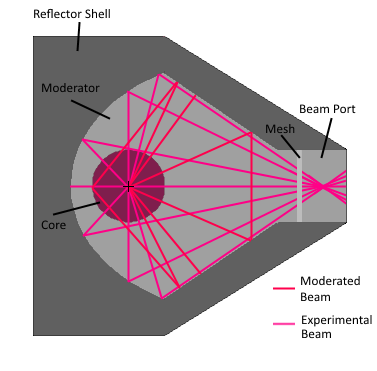
\includegraphics[width=0.85\textwidth]{design-02.png}
\caption{GOFR design}
\label{fig:design2}
\end{figure}
